\subsection{Pandas Dataframe operations}
A dataframe can be thought of as a list within a list supporting access in more meaningful ways compared to using indices.

\begin{tabular*}{\linewidth}{m{0.45\linewidth} | m{0.45\linewidth} |}
    \textbf{Example dataframe} & \textbf{Change Index Column}\\
    \hline
    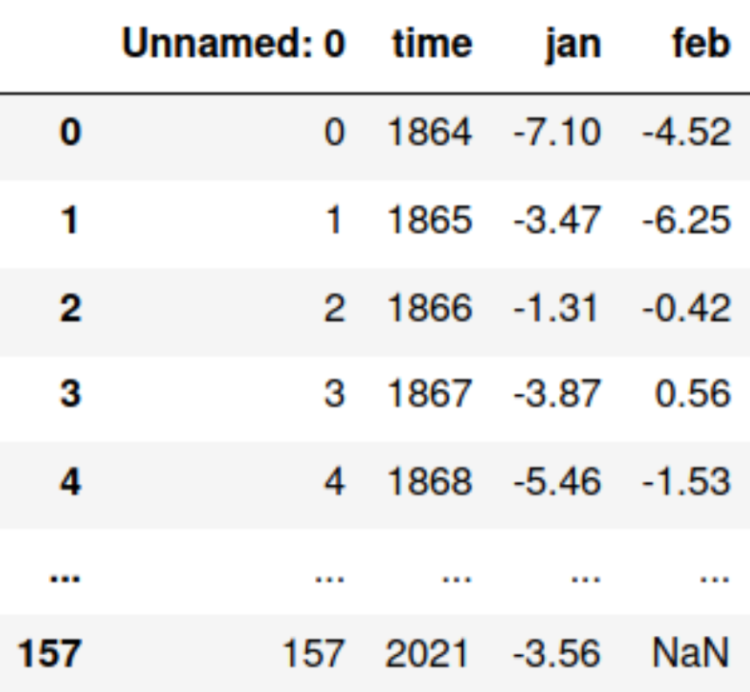
\includegraphics[width=\linewidth]{src/10_pandas/images/pd_dataframe_index.png} & 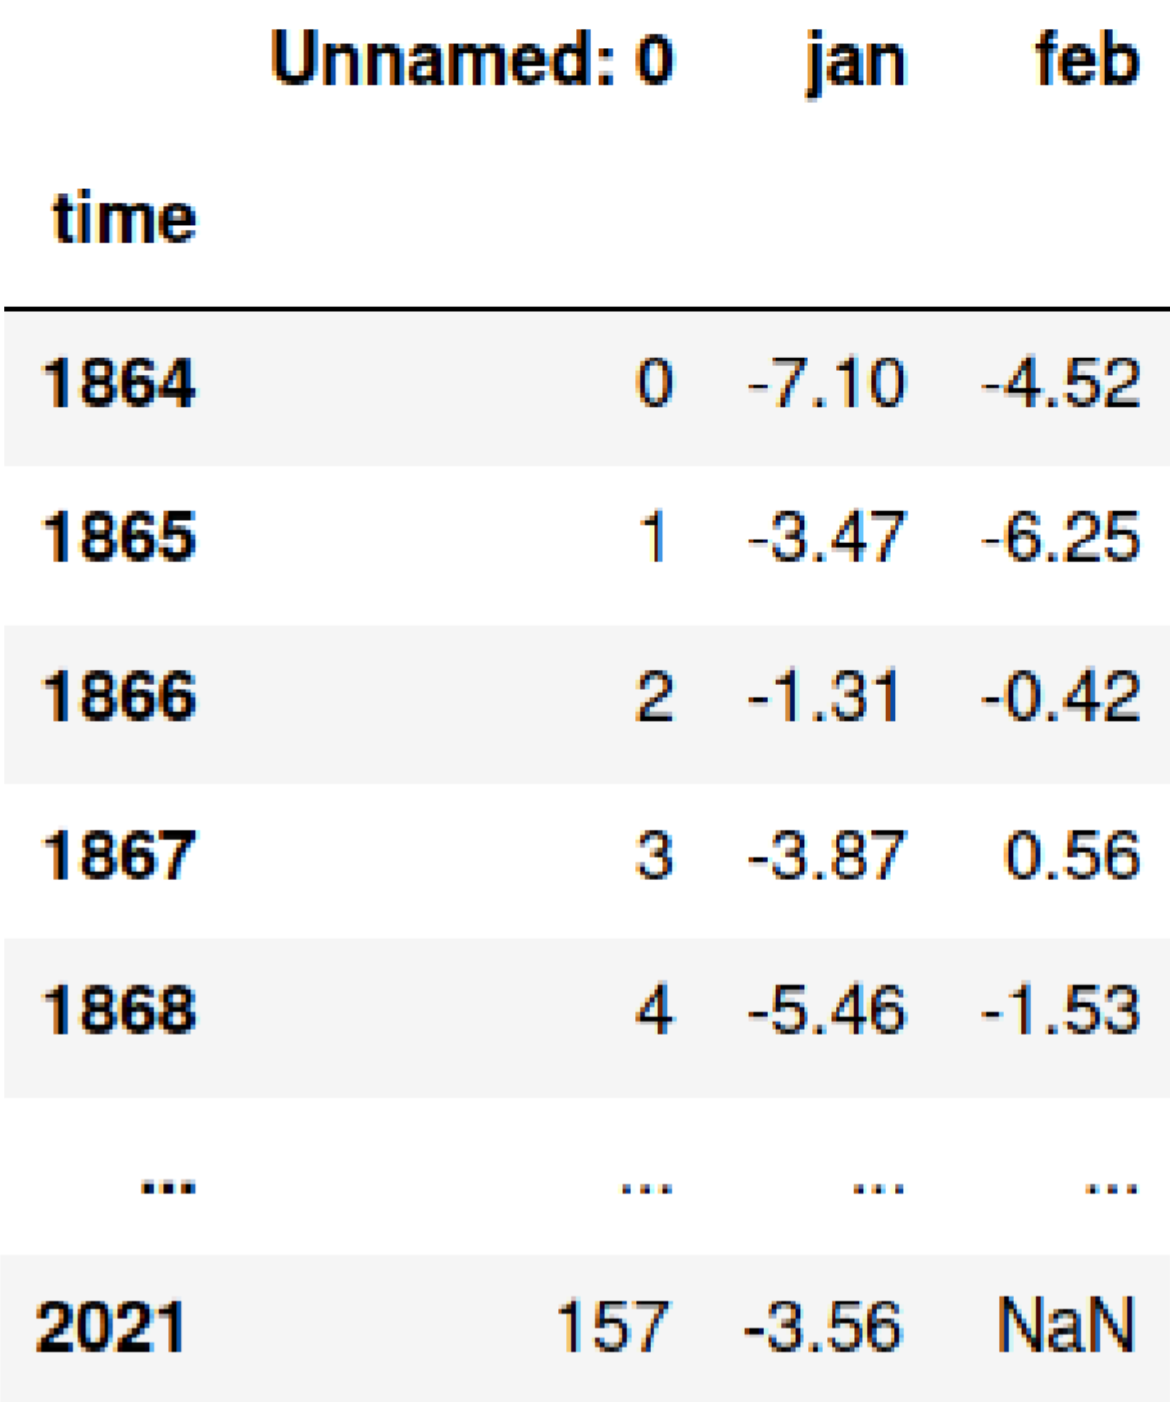
\includegraphics[width = 0.8\linewidth]{src/10_pandas/images/pd_dataframe_time.png}\\
    table of the climate, entries accessible via index. The leftmost column is known as the "index column". & \lstinputlisting{src/10_pandas/code/change_index.py} table of the climate, entries accessible via time
\end{tabular*}
 
{\centering\underline{\textbf{Rename Columns}} \par}
\begin{lstlisting}
climate = climate.rename(columns={"old_index_name":"new_index_name", ...})
#renames the "old_index_name" column to "new_index_name"
\end{lstlisting}
rename all columns (len(data.columns) = number of colums must be true)
\begin{lstlisting}
data.columns = ["Date", "January", "February", ...]
\end{lstlisting}

{\centering\underline{\textbf{Access Dataframe Elements}} \par}
\lstinputlisting{src/10_pandas/code/access_elements.py}

{\centering\underline{\textbf{Filter Dataframes}} \par}
Filter rows:
\begin{lstlisting}
climate[climate["jan"]>2]
#filters out the rows with values in the "jan" column #less than 2
\end{lstlisting}
• Example: All entries in "jan" with values more than 2:
\begin{lstlisting}
climate["jan"][climate["jan"]>2]
\end{lstlisting}

{\centering\underline{\textbf{Dealing with Invalid Data}} \par}
Convert all the values in a column to numeric:
\begin{lstlisting}
data[column] = pd.to_numeric(data[column], errors="coerce")
#converts all the values to numeric values. #errors="coerce" -> converts values which cannot be #converted to NaN.
\end{lstlisting}
Delete all rows containing NaN entries:
\begin{lstlisting}
data.dropna(axis = 0, how="any")
#how="any" -> delete row if any value is NaN.
#how="all" -> delete row if all values are NaN
#axis = 1 -> delete column instead of row
\end{lstlisting}
• Fill all entries containing NaN with a value:
\begin{lstlisting}
data.fillna(0) #fill any NaN entries with 0
\end{lstlisting}

{\centering\underline{\textbf{Modify Dataframes}} \par}
Add a column:
\begin{lstlisting}
climate["new_col"] = climate["time"] + climate["jan"] 
#"new_col" is a new column whose values are #those of the "time" and "jan" column added
\end{lstlisting}
Delete a column:
\begin{lstlisting}
climate = climate.drop(columns=["time"])
#delete the "time" column
\end{lstlisting}
Add a row:
\begin{lstlisting}
d = {"mar":34, "jan":23}
climate.append(d, ignore_index=True)
#adds another row with the values 34 for "mar" and 23 for #"jan". Other entries are NaN
\end{lstlisting}
Delete a row:
\begin{lstlisting}
climate = climate.drop(climate.index[0]) 
#deletes row 0
\end{lstlisting}
Transpose the dataframe:
\begin{lstlisting}
climate = climate.T
\end{lstlisting}

{\centering\underline{\textbf{Analyse Data}} \par}
Sum of all the entries in each column (type: Series):
\begin{lstlisting}
climate.sum()
\end{lstlisting}
Maximum of all the entries in each column (type: Series):
\begin{lstlisting}
climate.max()
\end{lstlisting}
Create a dataframe summarizing the max and sum for each column:
\begin{lstlisting}
climate.agg(["max","sum"])
#A dataframe containing the same columns as climate
#with row 0 containing the max of the column and row 1 #containing the sum of the column. The strings in the 
#list should be names of valid pandas Series functions. 
\end{lstlisting}
Get statistical information for each column (type: Dataframe):
\begin{lstlisting}
climate.describe()
#includes a variety of statistical measures
\end{lstlisting}
Sort a dataframe according to entries in a specific column(s):
\begin{lstlisting}
climate = climate.sort_values(["time", "jan"], ascending=False)
#sorts the rows by "time" in descending order. If two #entries for "time" are equal, then the rows are sorted #by "jan"
\end{lstlisting}
Split a dataframe into groups based on a specified column and perform a computation on each group:
\begin{lstlisting}
data.groupby("column").sum() 
#groups data based on the entries for "column" and #calculates the sum for each group.
data.groupby("column").max()
#groups data based on the entries for "column" and #calculates the max for each group.
\end{lstlisting}